\documentclass[12pt]{article}
%\usepackage[utf8]{inputenc}
%\documentclass[UTF8]{ctexart}
%\usepackage[UTF8, heading = false, scheme = plain]{ctex}
\usepackage{geometry}
%geometry{a4paper,scale=0.9}
\geometry{a4paper,left=1cm,right=1cm,top=1cm,bottom=2cm}
\usepackage{amsfonts}
\usepackage{color}
\usepackage{url}
%\usepackage{biblatex}
\usepackage{amsmath}
\usepackage{amssymb}
\usepackage{latexsym}
\usepackage{cite}
%\addbibresource{ref.bib}
%\bibliography{ref.bib}
\usepackage{caption}
\usepackage{graphicx, subfig}
\usepackage{float}
%\usepackage[fontset=ubuntu]{ctex}
%\usepackage{fontspec}
\usepackage{xeCJK}
%\usepackage[colorlinks,
%anchorcolor=black,
%citecolor=black]{hyperref}
%\setmainfont{SimSun}
\usepackage[section]{placeins}
\usepackage{enumitem}
\usepackage{framed}
\usepackage[framemethod=TikZ]{mdframed}
\usepackage{indentfirst}
\usepackage{setspace}%使用间距宏包
\linespread{1.5}

\title{因果推断概述\cite{Causal_Inference_Simply_Introduction}\cite{Talk_About_Causal_Inference_Part_1}}
\author{leolinuxer}
%\date{June 2020}

\begin{document}
%\setlength{\parindent}{0pt}
\maketitle
\tableofcontents

\section{因果性与相关性}
\subsection{因果性与相关性的比较}
事件/变量之间的关系,最主要的有\textbf{相关性}和\textbf{因果性}。
\begin{itemize}
\setlength{\itemsep}{0pt}
\setlength{\parsep}{0pt}
\setlength{\parskip}{0pt}
    \item 相关性是指在观测到的数据分布中,$X$与$Y$相关,如果我们观测到$X$的分布,就可以推断出$Y$的分布;
    \item 因果性是指在操作/改变$X$后,$Y$随着这种操作/改变也变化,则说明$X$是$Y$的\textbf{因cause};
\end{itemize}

在常用的机器学习算法中,关注的是特征之间的相关性,而无法去识别特征之间的因果性,而很多时候在做决策与判断的时候,我们需要的是因果性。

举个例子,我们会发现在学校中,近视的同学成绩更好。近视和成绩好之间有强相关性,但显然近视不是成绩好的原因。而我们想要提升学生成绩,自然需要找到因,否则就会通过给学生戴眼镜的方式来提高成绩。这个例子是很明显地可以区分出相关与因果的,但是也有很多难以区分的,如经常喝葡萄酒的人寿命更长,是因为葡萄酒确实能延长寿命,还是因为能经常喝的人通常更富有,享有更好的医疗条件。再比如:
\begin{itemize}
\setlength{\itemsep}{0pt}
\setlength{\parsep}{0pt}
\setlength{\parskip}{0pt}
    \item 在 feeds 流里刷到一个新推荐策略的内容的用户留存更高,他们的高留存是因为这个推荐策略导致的吗,这个策略究竟对留存的提升有多大效果?
;
    \item 上周投放了某游戏广告的用户登录率更高,他们的高登录率有多大程度是由广告带来的,有多大程度是由于他们本身就是高潜力用户?
\end{itemize}


\subsection{识别因果的必要性}
有些时候,我们通过统计学方法或者机器学习算法得到的特征之间的相关性,就足以为我们的验证、决策提供指导,比如,我们通过数据发现,用户曝光的图片越多,留存越高,我们不需要知道这之间是否有复杂的因果关系,只需要通过简单的ABtest来检验更多的曝光是否有效果即可。

在这些例子中,本质上,我们都是想要分析一个干预(treatment)对一个结果(outcome)有怎样的影响,想要探究其中的因果效应。大家熟悉的 A/B Test 是回答上面这些问题的黄金方式。但是,A/B Test 也有一定的局限性,例如:
\begin{itemize}
\setlength{\itemsep}{0pt}
\setlength{\parsep}{0pt}
\setlength{\parskip}{0pt}
    \item 药物是否有效、政策是否有效,这种问题无法做 ABtest;
    \item 新的推荐算法是否有效,ABtest成本高(不好的用户体验等);
    \item 需要花一定的时间实现,比较耗费人力;
    \item 需要占用足量的随机流量,并且需要持续一段时间以收集数据;
    \item 当可做 A/B Test 的选择太多时,往往难以全部都进行尝试。
\end{itemize}

因此,面对这种特殊的问题,我们需要\textbf{从已有的数据}中推断出变量间的因果性。

\section{因果推断推什么}
\begin{mdframed}[
linecolor=black!40,outerlinewidth=1pt,roundcorner=.5em,innertopmargin=1ex,innerbottommargin=.5\baselineskip,innerrightmargin=1em,innerleftmargin=1em,backgroundcolor=gray!5,
%backgroundcolor=blue!10,%userdefinedwidth=1\textwidth,%shadow=true,%shadowsize=6,%shadowcolor=black!20,%frametitle={The \textit{two-step} model of XMCD:},%frametitlebackgroundcolor=cyan!40,%frametitlerulewidth=10pt
]
一些定义:

\textbf{因果关系(Causality)的定义:T causes Y if and only if changing T leads to a change in Y,while keeping everything else constant. \cite{Causal_Inference_and_Stable_Learning}}

\textbf{因果效应(Causal effect)的定义:Causal effect is defined as the magnitude by which Y is changed by a unit change in T.}

\textbf{结构化因果模型(Structural Causal Model):A graphical model to describe the causal mechanisms of a system}
\begin{figure}[H]
    \centering
    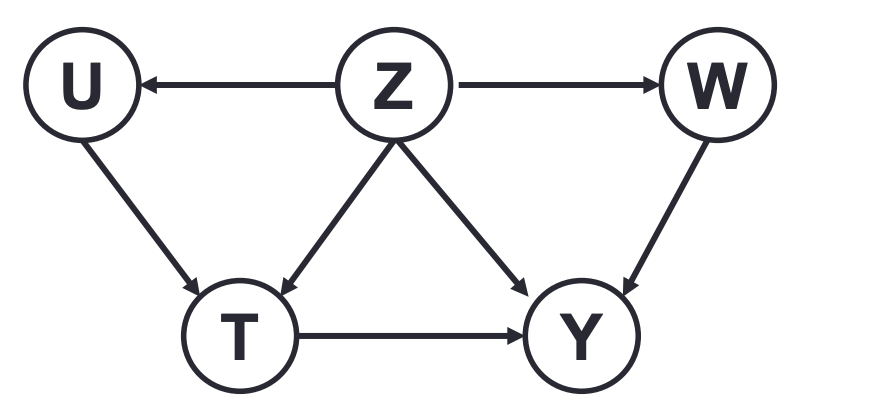
\includegraphics[width=0.5\textwidth]{fig/Causal_Inference_and_Stable_Learning-Causal-Model.png}
\end{figure}
\end{mdframed}


因果推断用的最多的模型有两个。一个是著名的统计学家 Donald Rubin 教授在 1978 年提出的 “潜在结果模型”(potential outcome framework),也称为 Rubin Causal Model(RCM)。另一个是 Judea Pearl 教授在 1995 年提出的因果图模型(Causal Diagram)。这两个模型实际上是等价的。

首先,我们需要定义一些符号:
\begin{itemize}
\setlength{\itemsep}{0pt}
\setlength{\parsep}{0pt}
\setlength{\parskip}{0pt}
    \item \textbf{干预 (treatment) $T$}:一般我们考虑二值干预,用 $T_i \in \{0,1\}$ 来指示用户是否受到了某种干预,例如是否被投放了某广告、是否被灰度了某功能。在 A/B Test 中,实验组的用户都受到了某种处理,他们都有 $T_i=1$。

    \item \textbf{潜在结果(potential outcome)$\{Y_{i0}, Y_{i1}\}$}:对每个用户 $i$,他们对于是否受到干预分别有两个潜在结果 $Y_{i0}$ 和 $Y_{i1}$。例如,$Y_{i0}$ 和 $Y_{i1}$ 分别表示假如一个用户没有被投放游戏广告和被投放时是否会登录游戏。
    
    \item \textbf{观察结果(observed outcome)$Y$}:当一个用户没有受到干预时($T=0$),我们将会观察到 $Y=Y_{i0}$,当一个用户受到干预时我们将会观察到 $Y=Y_{i1}$。
\end{itemize}

在因果分析中,我们通常比较关心以下两种 “因果效应”。为了符号简洁,接下来不再特意标注出代表用户的下标 :
\begin{itemize}
\setlength{\itemsep}{0pt}
\setlength{\parsep}{0pt}
\setlength{\parskip}{0pt}
    \item \textbf{平均因果效应 (Average Treatment Effect,简称 ATE)}: $ATE=E[Y_1 - Y_0]$。$ATE$ 为干预对所有人的平均因果效应。

    \item \textbf{干预组的平均因果效应(Average Treatment Effect on the Treated,简称 ATT)}:$ATE=E[Y_1 - Y_0|T = 1]$。$ATT$ 为干预对受到干预的人的平均因果效应。
\end{itemize}

以游戏广告投放为例,我们举一个例子如下表,这个例子接下来还会反复使用。假如我们可以同时观测到两个潜在结果(\textbf{尽管这是不可能的}),我们可以算出 
\begin{figure}[H]
    \centering
    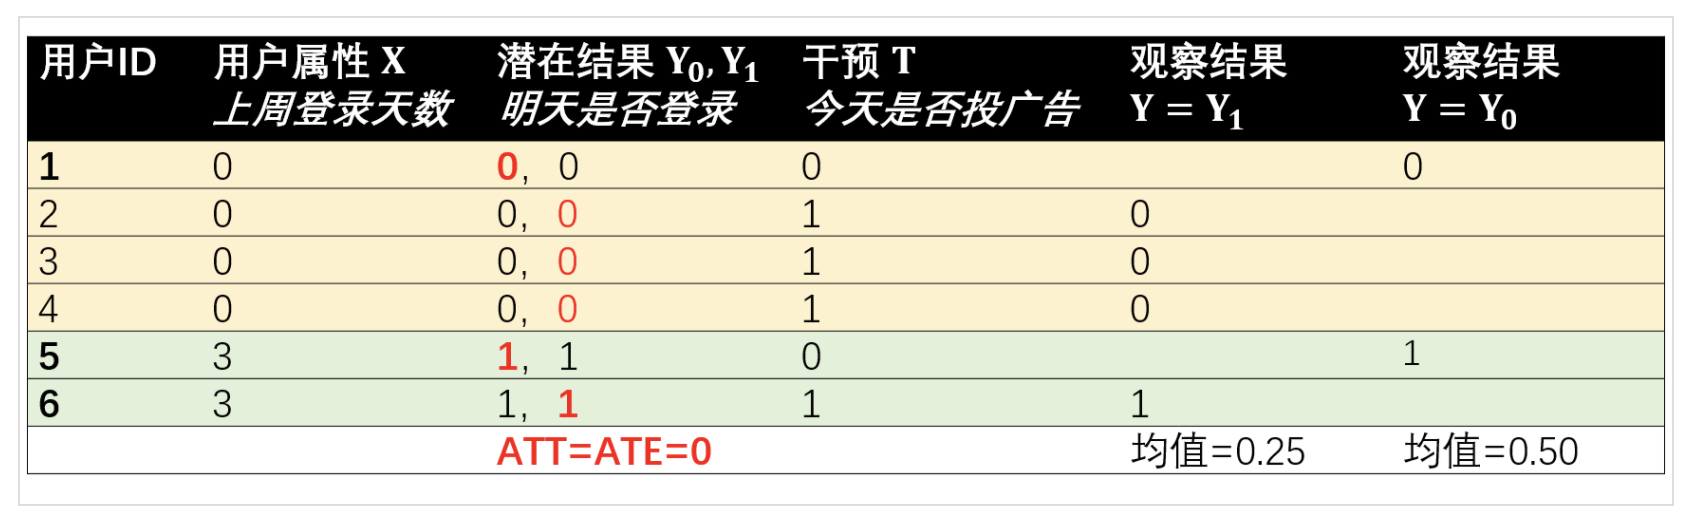
\includegraphics[width=1\textwidth]{fig/CasualInference-Game-Ad-1.png}
\end{figure}

当我们尝试直接从观察结果$Y$  统计 $ATE$ 或者 $ATT$ 时,我们就会遇到一个问题:对于每一个用户,我们并不能同时观测到两个潜在结果。这个问题是因果推断的一个核心问题、核心难点。

\begin{mdframed}[
linecolor=black!40,outerlinewidth=1pt,roundcorner=.5em,innertopmargin=1ex,innerbottommargin=.5\baselineskip,innerrightmargin=1em,innerleftmargin=1em,backgroundcolor=gray!5,
%backgroundcolor=blue!10,%userdefinedwidth=1\textwidth,%shadow=true,%shadowsize=6,%shadowcolor=black!20,%frametitle={The \textit{two-step} model of XMCD:},%frametitlebackgroundcolor=cyan!40,%frametitlerulewidth=10pt
]
\textbf{因果推断的核心思想在于\textcolor{red}{反事实推理counterfactual reasoning},即在我们观测到$X$和$Y$的情况下,推理如果当时没有做$X$,$Y'$是什么。}
\end{mdframed}

因果推断的目的是要判断因果性,即计算\textbf{因果效应}(有无$X$的情况下$Y$值的变化量)。在进行反事实推理后,可得出\textbf{因果效应}$e = |Y - Y'|$,进而判断因果性。

实际上,对于一个对象,我们永远只能观察到$Y$和$Y'$的其中一个,因果推断所做的就是从已有数据中估计因果效应,所以我认为因果推断的本质是对因果效应的估计。

A/B Test 提供了解决这个核心问题的完美方案,让我们通过简单的公式看看为什么。在做 A/B Test 时,我们一般直接统计实验组和对照组的指标差异。
根据 $ATT$ 的定义,我们可以得到如下公式推导
$$
ATT = E[Y_1 - Y_0 | T=1] = (E[Y_1|T=1] - E[Y_0|T=0]) - (E[Y_0|T=1] - E[Y_0|T=0]) = \hat{ATT} + bias
$$

其中,$\hat{ATT}$定义为:
$$
\hat{ATT} = E[Y_1 | T = 1] - E[Y_0|T=0]
$$

这里的 bias,根据定义来看,是实验组和对照组的潜在结果 $Y_0$ 的差异。在 A/B Test 中,我们假设实验组和对照组是随机划分的,因此 bias 为 0。因此,根据 A/B Test 计算的 $\hat{ATT}$ 就是 $ATT$ 的无偏估计。即$\hat{ATT}$就是我们的估算方式。

在日常工作中,并非所有数据分析都有 A/B Test 撑腰。我们往往需要通过观察历史数据完成分析,这类分析称为 “观察性研究”。在观察性研究中,失去了 “随机流量” 的撑腰,现实就没有那么美好了。这时,如果我们直接比较两组用户指标上的差异得到 $\hat{ATT}$,它和真实的 $ATT$ 之间是存在一个非零的 bias 的,我们无法根据  $\hat{ATT}$ 下一个科学可靠的结论。 例如,在之前使用的广告投放的例子中,假设我们直接比较 $T=1$ 和 $T=0$ 两组用户的观测结果 $Y$的差异,会造成投放广告造成登录率从 50\% 下跌到 25\% 的错觉,这并不是真实的 $ATE$ 和 $ATT$。


\section{因果效应的可识别性}
在观察性研究中,借助什么样的数据可以推出可靠的因果效应($ATE$ 或 $ATT$)呢?具体来说,假如我们对每个用户有一系列干预前的指标(pre-treatment variables) $X$、有干预 $T$、有观察结果 $Y$,我们能不能推断出 $T$ 对 $Y$ 的因果效应?
这个问题就是因果推断的可识别性(identifiability)问题。可识别性依赖于几个假设,这些假设通常被称为 causal assumption。下面我们一个一个来看看。

\subsection{Stable Unit Treatment Value Assumption (SUTVA)}
SUTVA 假设用户之间是相互独立的,无互相干扰。SUTVA 保证个体的潜在结果只和他自己有关、最终观察到的结果也只和他自己有关。值得注意的是,社交网络上的实验理论上都很难完完全全保证 SUTVA,但是对于大部分社交属性不强的实验,一般还是假设 SUTVA 基本成立。

\subsection{Ignorability}
Ignorability 假设对于 pre-treatment 变量 $X$ 一样的人群,是否接受处理和潜在结果相互独立:$Y_0, Y_1 \bot T|X$。$\bot$ 表示独立性。

这个假设比较难以理解,我们套用之前举的广告投放的例子看看。在这个例子中,我们倾向于给历史登录天数少的用户投放广告,$X$ 和 $T$ 是负相关的。同时,历史登录天数越多,未来登录率也越高,即 $X$ 和潜在结果 $Y_0$ 和 $Y_1$ 都是正相关的。在这份数据里,$(Y_0, Y_1)$ 和 $T$ 并不独立。但是,对于 $X$ 取值一样的用户,是否看到广告可以看做是随机的,ignorability 成立。

Ignorability 这个假设还有很多其它的名字,例如 no unmeasured confounders assumption 和 Conditional Independence Assumption (CIA)。

\subsection{Consistency}
Consistency 假设潜在结果和观察到的结果是一致的,即当 $T = t$时 $Y = Y_t$。这个假设一般可以认为是成立的。

\subsection{Positivity}
Positivity 假设要求 treatment assignment 有一定随机性,要求对于$X$ 的所有取值都有 $ 0 < Pr[T=1|X=x] < 1$。如果这个假设不成立,我们是无法下结论的。例如当一部分用户不可能被投放广告时,我们无法通过历史数据分析广告对他们的效果。当 positivity 假设不成立时,我们往往需要考虑去除一些特殊用户群。

Positivity 这个假设也有些其它的名字,常见的有 common support 和 overlap。

A/B Test 满足上面的每一个假设。在观察性研究中,SUTVA、ignorability 和 consistency 这三个假设都是无法验证的(untestable)。有时我们可以通过一些经验或是数据判断出这些假设明显不成立,但是我们没有办法可以证明这些假设成立。

\section{一些因果推断的方法}
\subsection{随机实验Randomization}
\subsubsection{A/B Test}
以推荐算法为例,判断推荐算法是否有效,ABTest通过将用户随机分为两组,分别应用不同的算法,通过判断两组用户点击率的差异来估计因果效应。通过随机分组,排除了混淆变量的影响。

A/B Test实际上是判断因果性的很有效的方法,但有时候成本过高无法采用,如这里的推荐算法——
\begin{itemize}
\setlength{\itemsep}{0pt}
\setlength{\parsep}{0pt}
\setlength{\parskip}{0pt}
    \item 可能新的推荐算法太差导致用户流失;
    \item 如果有很多新的算法要测试,A/B Test效率较低;
\end{itemize}

\subsubsection{多臂老虎机 Multi-armed bandits}
针对上述问题,另一种随机实验方法是强化学习中的多臂老虎机,实际上是\textbf{对explore和exploit的平衡}。
\begin{itemize}
\setlength{\itemsep}{0pt}
\setlength{\parsep}{0pt}
\setlength{\parskip}{0pt}
    \item explore,随机选择一个动作,在上面的问题中是随机选择一个算法;
    \item exploit,选择收益最高的动作,在上面的问题中是选择当前效果最好的算法;
\end{itemize}

通过某种规则(e-greedy等)重复上述过程,优点是可以同时测试多种算法,并且每个用户都能使用到最好的算法,减少流失可能性。缺点是效果难以评估,也很难让用户按照我们的想法行动。

\subsection{自然实验Natural Experiments}
理想的实验需要:\textbf{随机分配(分组)、人为干预(施加不同的treatment)、结果比较}。

自然实验实际上是一种\textbf{观察性研究},满足上述三个条件中的两个,是指不加干预地、实验对象\textbf{“自然”}地分为若干组,对实验对象的结果进行观察比较。

显然自然实验法的关键在于,实验对象是否能“自然”/随机地分组。比如,将是否民主将国家分为两组,探究制度与国家对外战争的关系。但是在这里,是否民主不是随机的分给各个国家,所以无法满足自然实验所需的随机分配原则。

\subsubsection{断点回归Regression discontinuity}
断点回归是自然实验中的一种观察方法,简单理解就是在回归过程中,观察在临界点处是否出现断层/断点。

举一个简单的例子,假设现在有一个产品,收集500个金币后就可以得到一个勋章,现在要判断有无勋章对用户在线时长的影响。断点回归法观察金币在500附近的用户,如497到502,观察【接近500但小于500(无勋章)】与【接近500但大于500(有勋章)】的用户在线时长是否有显著区别,若有,说明有勋章很可能会增加用户的在线时长。

\subsubsection{工具变量Instrumental Variables}
对于要判断因果关系的两个变量间,如果存在其他混淆变量,在计量经济学中采用工具变量的方法解决。

以下述关系为例,要判断对APP1的访问,是否会导致对APP2的点击。实际上由于APP1和APP2之间的需求关系,误差项与解释变量相关,即计量经济学中的内生性。
\begin{figure}[H]
    \centering
    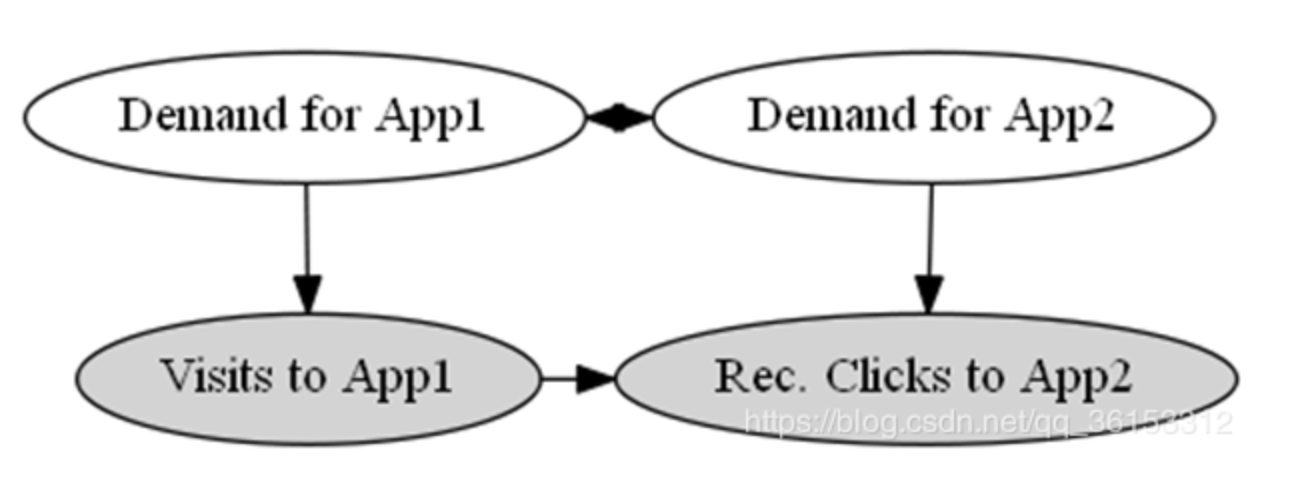
\includegraphics[width=0.8\textwidth]{fig/CasualInference-APP-User-Example.png}
\end{figure}

\textbf{引入工具变量的目的是为了让误差项与解释变量不相关}。具体地,通过找到一个变量,满足与解释变量相关且与误差项无关,那在引入这一变量之后,解释变量变化的部分就与误差项无关。

同样是上面的例子,假设某一天有个活动,下载APP1的人有奖励,这个活动与解释变量相关,但不会影响到APP2的需求,那根据多出来的APP1访问量与多出来的APP2点击率就不再受到需求关系的影响,就可以判断对APP1的访问,是否会导致对APP2的点击。
\begin{figure}[H]
    \centering
    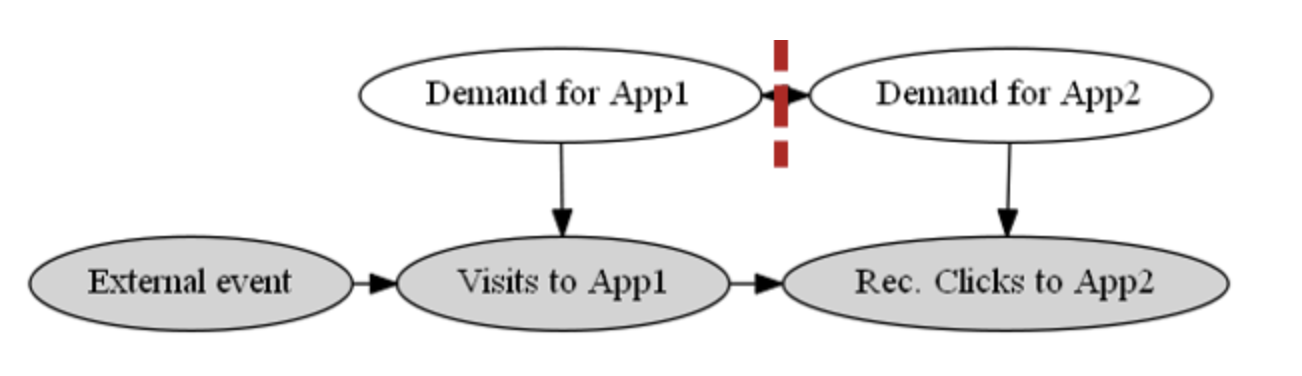
\includegraphics[width=0.8\textwidth]{fig/CasualInference-APP-User-Example2.png}
\end{figure}

\subsection{Conditioning}
\subsubsection{分层Stratification}
分层的核心思想是控制条件变量,一般步骤如下:
\begin{itemize}
\setlength{\itemsep}{0pt}
\setlength{\parsep}{0pt}
\setlength{\parskip}{0pt}
    \item 尽可能完整的绘制出变量之间的因果图
    \item 选择影响要判断因果性的变量的条件变量
    \item 对用户进行分层/分组,满足组内的用户条件变量取值一致(上层的变量将全部不需要再考虑,类似贝叶斯网络中的d分隔)
    \item 比较两组用户的输出,计算因果效应
\end{itemize}
这种方式有点类似要找到相似的用户,当条件变量很多的时候,这种方法很难实现,很难找到很多条件变量都相同的用户,即使找到也会使得分组偏小。

\subsubsection{倾向得分匹配Propensity score matching}
当条件变量很多的时候,可以考虑使用倾向得分匹配。

以推荐算法为例,当条件变量很多的时候,通过逻辑回归等方法对这些变量进行训练,并计算出一个倾向得分,在这里是用户被施加新算法的概率。因此倾向得分匹配的一般步骤如下:
\begin{itemize}
\setlength{\itemsep}{0pt}
\setlength{\parsep}{0pt}
\setlength{\parskip}{0pt}
    \item 尽可能完整的绘制出变量之间的因果图
    \item 选择影响要判断因果性的变量的条件变量
    \item 对用户进行分层/分组,满足组内的用户计算得出的倾向得分接近(上层的变量将全部不需要再考虑,类似贝叶斯网络中的d分隔)
    \item 比较两组用户的输出,计算因果效应
\end{itemize}

\subsection{Matching 方法详解}
假设我们有一份数据,我们判断几个 causal assumption 都是成立的,我们应该如何推断其中的因果效应呢?基于潜在结果模型,一套比较经典的因果效应推断方式是 Matching。Matching 这个方法从名字来看很直观,但是里头还是有一些套路的。

最最基本款的 Matching 是 Exact Matching。假设我们感兴趣的因果效应是 $ATT$,我们需要做的事很简单,对于每一个 $T=1$ 的用户,我们从 $T=0$ 的分组里找一个 pre-treatment 变量 $X$ 一模一样的用户,把他们配成对,找不到就放弃。配对过程结束后,一部分或者全部 $T=1$ 的用户找到了平行世界的自己,我们直接比较两组用户观察结果 $Y$ 的差异就可以得到结论。 继续使用之前提到的广告投放的例子,假设我们进行一个有放回的 Exact Matching,配对结果如下。估算的 $ATT$ 为 0。
\begin{figure}[H]
    \centering
    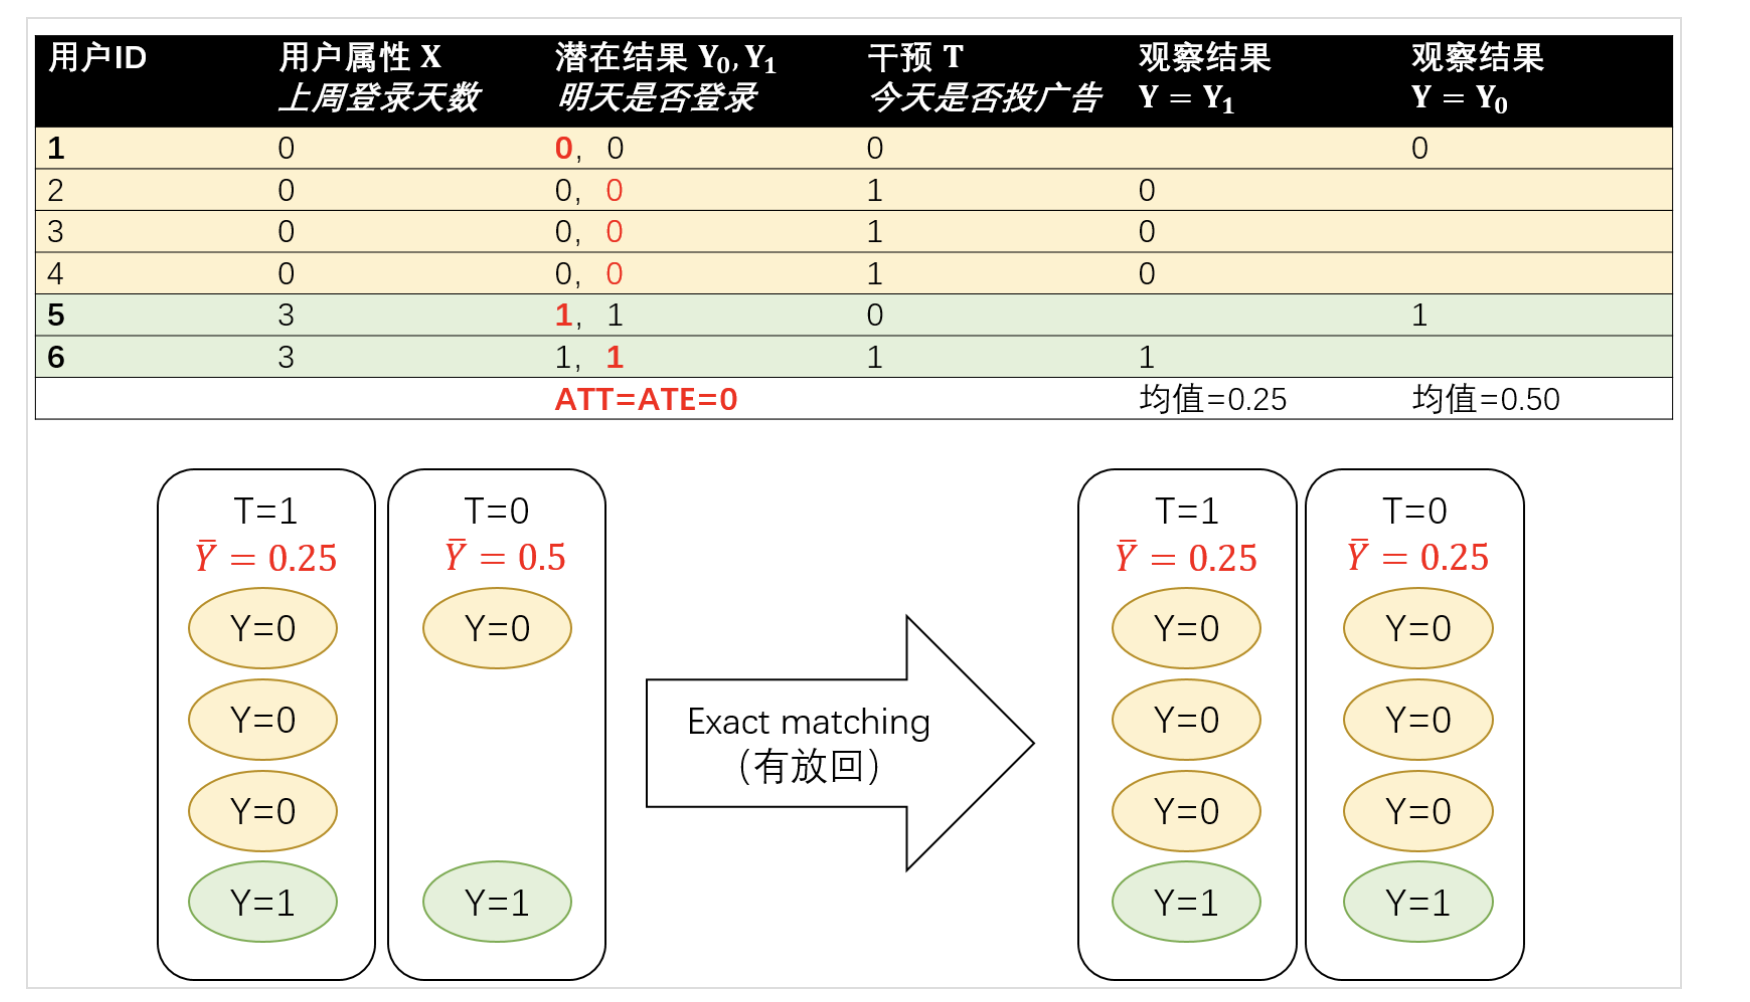
\includegraphics[width=1\textwidth]{fig/CasualInference-Game-Ad-2.png}
\end{figure}

Exact Matching 虽然直观,但是并不实用。“匹配用户的变量  $X$ 完全相等” 这个要求过于严格,随着变量 $X$ 的维度的增加,几乎不太可能有足量的匹配用户来下结论。

Exact Matching 的一个直观变种是 Distance Matching。我们可以对每一个 $T=1$ 的用户匹配一个距离最近并且不超过阈值的用户。这里 “距离” 如何定义、“阈值” 如何定义,也都需要更多的斟酌。另外,当我们通过距离来匹配时,其实是在潜意识里假设了变量 $X$ 的每一个维度都是同等 “重要” 的,这里也不一定科学。

为了科学有效地进行 Matching,一个经典的做法是 Propensity Score Matching,简称 PSM。在 PSM 方法中,我们首先对每一个用户计算一个倾向性得分(propensity score),定义为 $e(X)=Pr(T=1|X=x)$。接着我们根据倾向性得分将用户进行匹配 ,从而得到两个 $X$ 上看起来基本同质的用户组,然后统计得到 $ATT$。PSM 方法在实现上有许多值得深入介绍的地方,例如如何得到 “倾向性得分”、如何选择匹配方式(如一对一匹配、一对多匹配、分层匹配、有放回或无放回匹配)、如何衡量匹配质量等。关于更多 PSM 的细节,将会在下一篇文章里深入介绍。等不及的小伙伴也可以读一读参考资料([综述类 paper] Caliendo M, Kopeinig S. Some practical guidance for the implementation of propensity score matching[J]. Journal of economic surveys, 2008, 22(1): 31-72.)。

文献\cite{Causal_Inference_and_Stable_Learning}中有一个很好的Matching的例子:
\begin{figure}[H]
    \centering
    \caption*{对照组($T=0$)和实验组($T=1$),注意用户实际有不用的几类(绿色、深蓝色、浅蓝色)}
    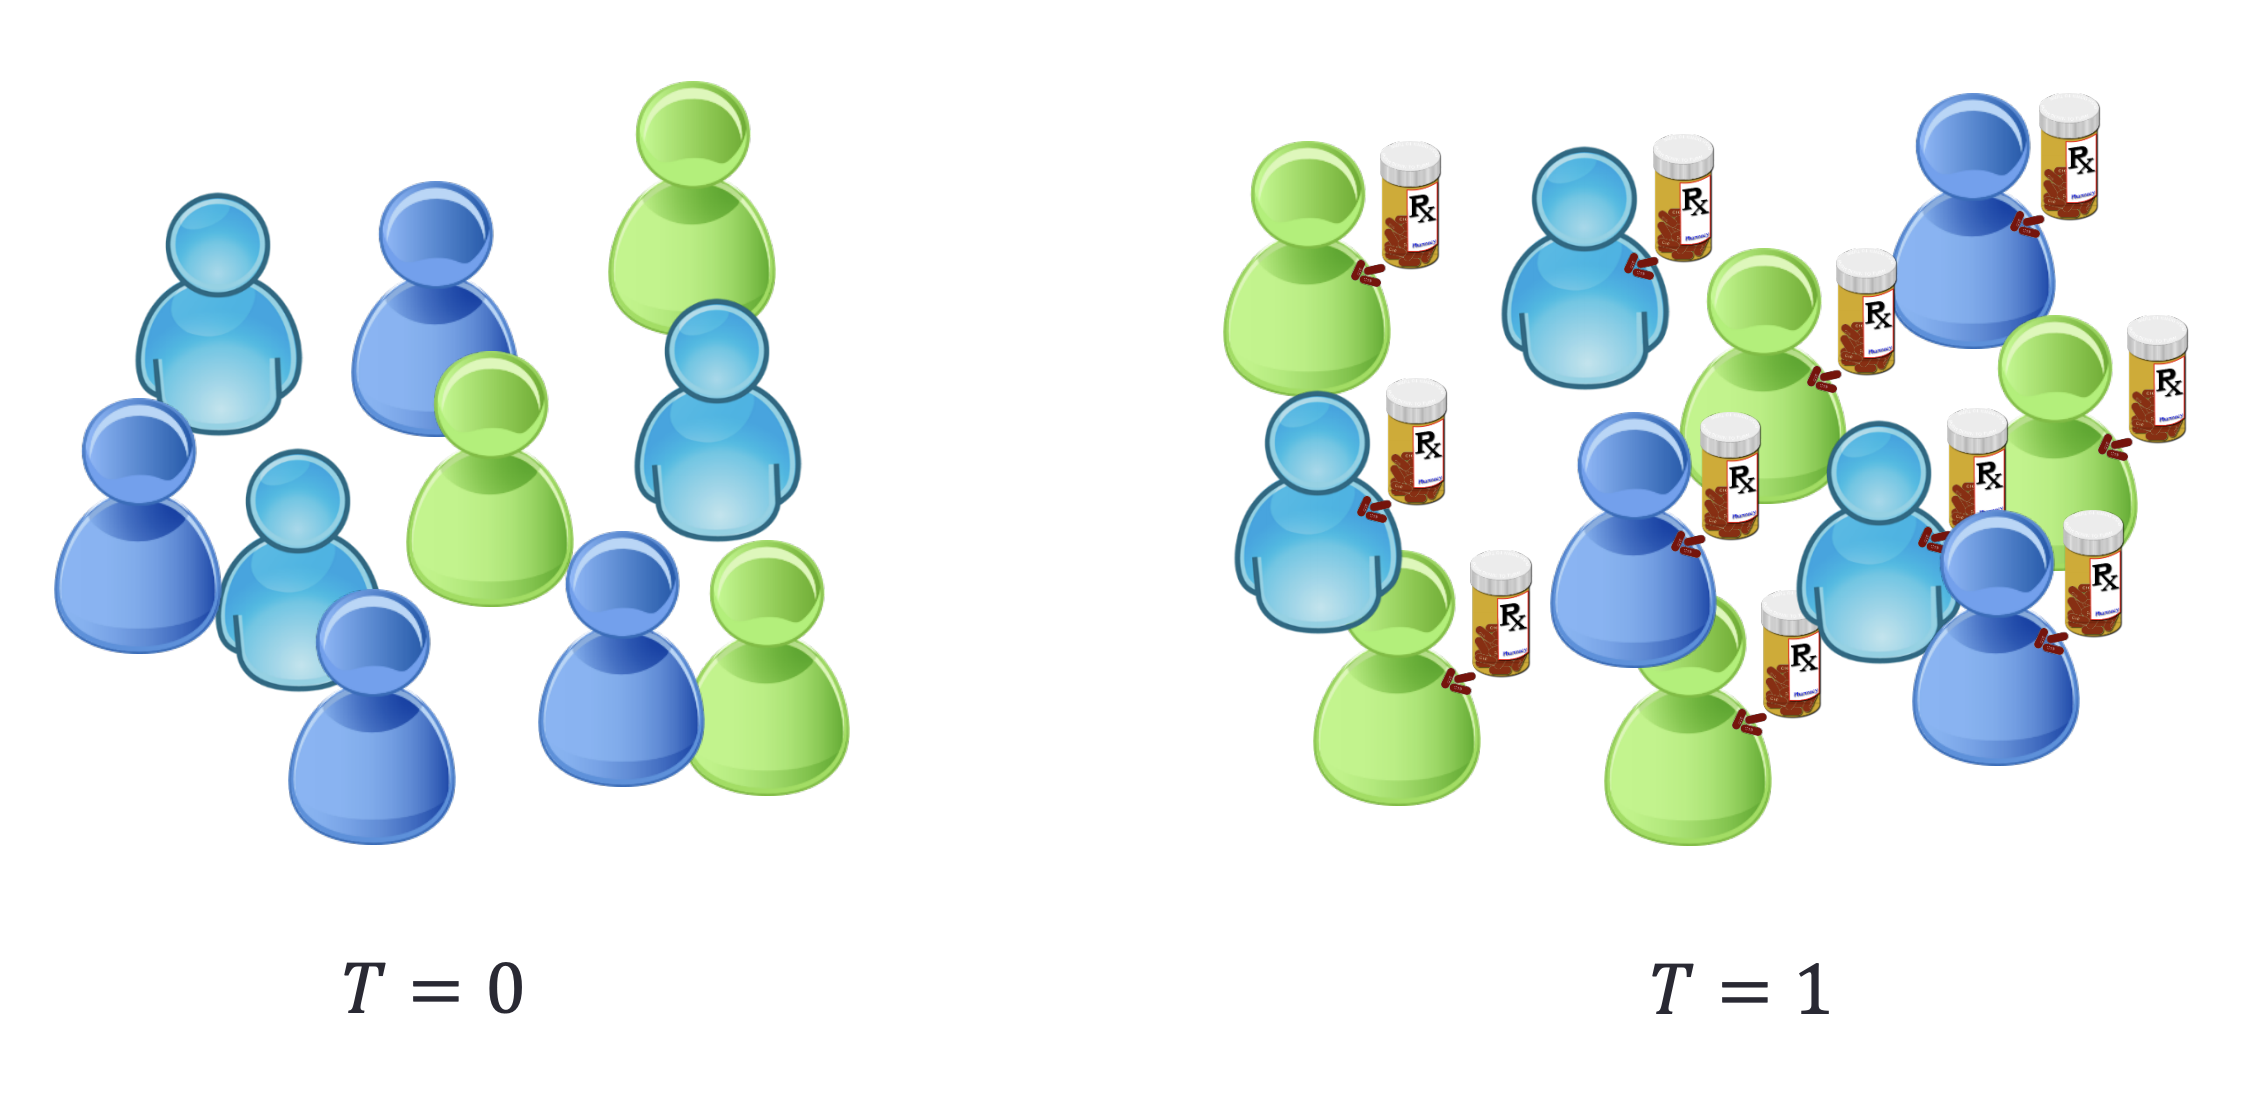
\includegraphics[width=0.8\textwidth]{fig/Causal_Inference_and_Stable_Learning-Matching-1.png}
\end{figure}

\begin{figure}[H]
    \centering
    \caption*{对用户进行 Matching,Matching 时的度量是:$Distance(X_i, X_j) \le \epsilon$;通过匹配,保证了同组的两个用户的其它特征都是基本相同的}
    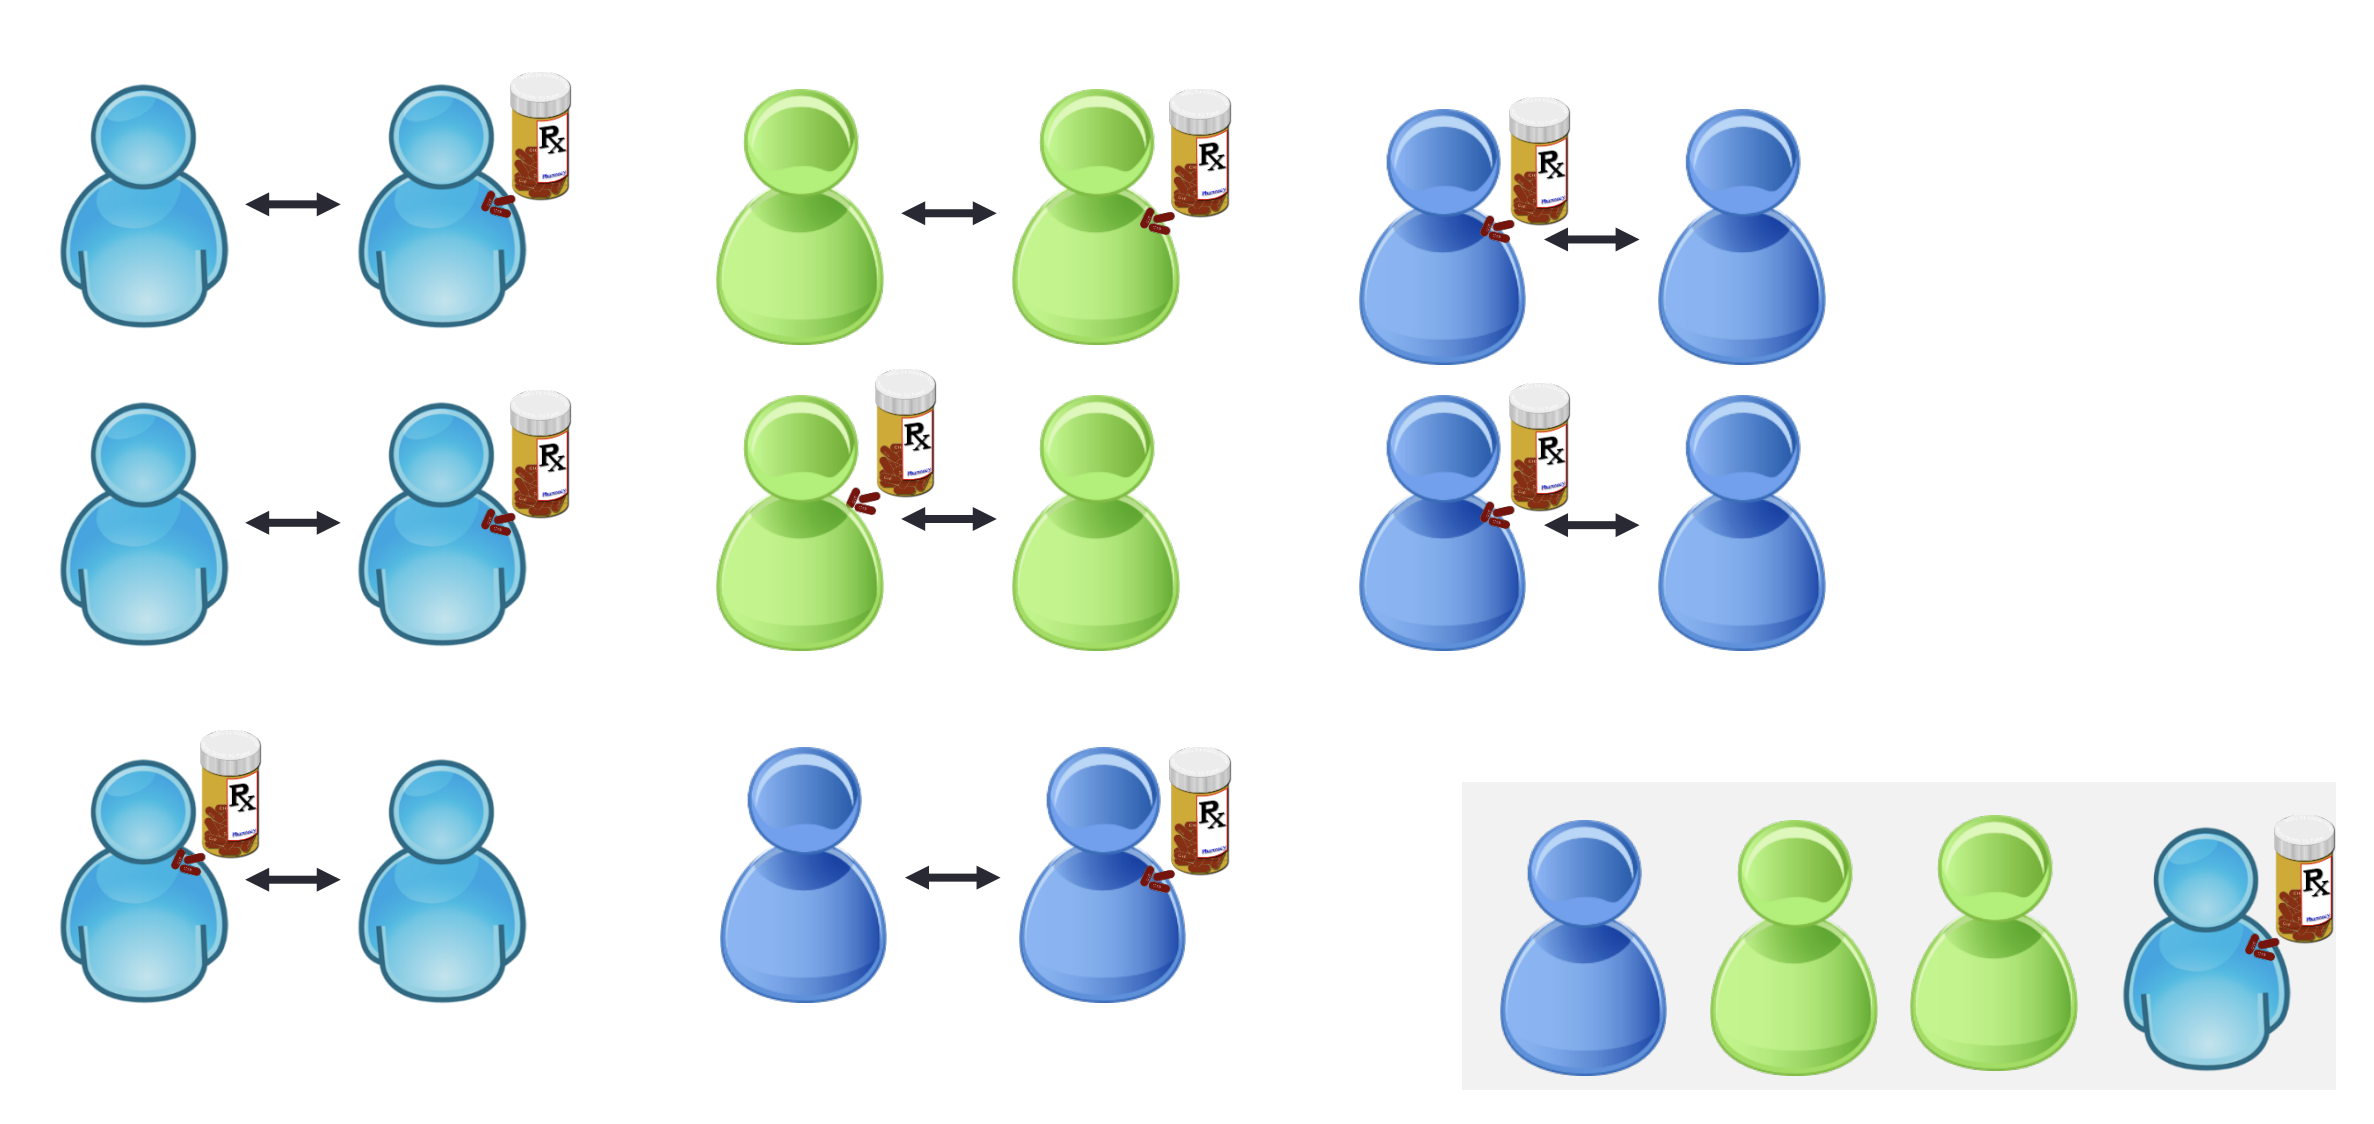
\includegraphics[width=0.8\textwidth]{fig/Causal_Inference_and_Stable_Learning-Matching-2.png}
\end{figure}


%\printbibliography
\bibliography{../ref}
\bibliographystyle{IEEEtran}
\end{document}